\documentclass[11pt,a4paper]{article}
\usepackage[utf8]{inputenc}
\usepackage{amsmath}
\usepackage{amsfonts}
\usepackage{amssymb}
\usepackage{graphicx}
\usepackage{paralist}
\usepackage{lmodern}
\usepackage[left=2cm,right=2cm,top=1.5cm,bottom=1.5cm]{geometry}
\usepackage[T1]{fontenc}
\usepackage[utf8]{inputenc}
\DeclareMathOperator*{\argmin}{argmin}
\DeclareMathOperator*{\argmax}{argmax}

\usepackage{xcolor}
\usepackage{tabto}
\usepackage{soul}
\date{\vspace{-14ex}}
%\date{}  % Toggle commenting to test

\begin{document}
\title{\Large \textbf{Oral Exam} Introduction to transportation planning}
\maketitle
\noindent\rule{16.9cm}{1pt}
\vspace{-3mm}
 \begin{flushright}
dr inż. Rafał Kucharski, KST, L-2, WIL, PK
\end{flushright}

\paragraph{Problems:}
\begin{enumerate}
\item How does your daily travel plan affect the transport system? Describe your plan and discuss, disaggregate it into the trips. Discuss how do you use the transport system. Do you partially cause congestion? Do the traffic jams affect you? 

\item Looking at your bus/tram today morning how would you describe travellers? Where they go to, what is their trip purpose, why did they choose this line? How would it change: 
\begin{enumerate}
\item during school holiday 
\item if the cars are all broken 
\item if there are huge traffic jams?
\end{enumerate}
\item Looking at your origin bus/tram stop in the morning how do you think the situation would change if: 
\begin{enumerate}
\item the new houses are built around for 2 000 people, 
\item there is a new office complex for 2 000 workers?
\end{enumerate}
\item Discuss the within day distribution of Home, Work, School and Other activities.
\item Discuss the within day distribution of Home-Work, Work-Home, Home-School, Work-Shopping trips.
\item List spatial variables that impact trip generation (where do people travel from and to)?
\item What is the meaning of the values in the OD matrices and how they are related to the trip generation (P/A)?
\item Imagine there are two options equally interesting, the first one costs 10zł, another costs 12zł. Estimate share of people selecting respective options: 
 \begin{enumerate} \item assuming deterministic (all-or-nothing) behaviour model, \item assuming probabilistic choice model, e.g. logit model. \end{enumerate}
\item How can we represent the transport network with a graph. Discuss arcs and nodes of road and transit network represented with a graph.
\item How does the volume (number of cars) impacts the travel time on an arc and how is it modelled in macroscopic static models?
\item Discuss the three key variables of traffic flow: speed, density and flow, use figure 1. as and example.
\item Describe the traffic situation shown on figure 2 and answer provided questions.
\end{enumerate}
\begin{figure}
\centering
\includegraphics[width=14cm]{funddiag}
\caption{Fundamental diagram of traffic flow}
\end{figure}
\begin{figure}
\centering
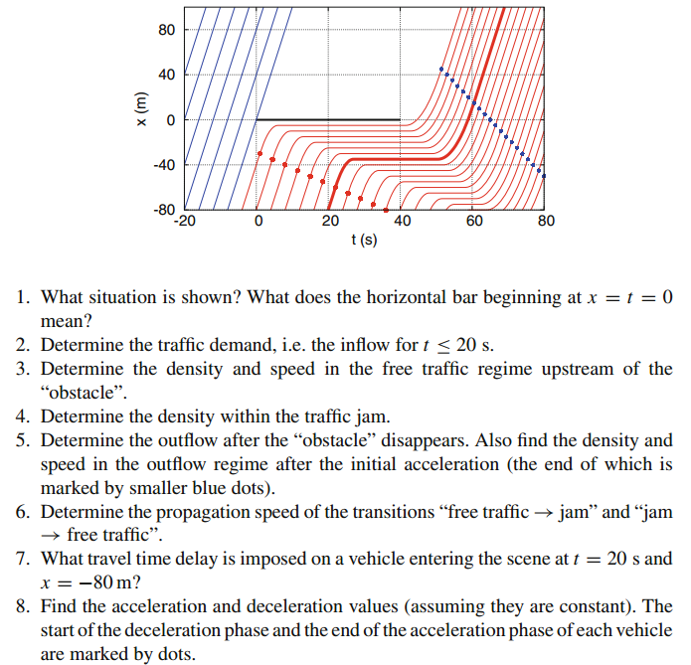
\includegraphics[width=14cm]{E1}
\caption{Space-time diagram of traffic queue}
\end{figure}
\noindent\rule{16.9cm}{1pt}
\end{document}

